\chapter{System Design and Methodology}
\label{chap:system-design-methodology}

\section{System Overview}
\label{sec:system-overview}

CliNotes is a web-based clinical documentation system designed to support the capture, transcription, structuring, review, and retrieval of medical consultation notes. The system addresses the practical problem that clinical documentation often requires a physician to divide attention between the patient encounter and the production of structured written records. In the implemented application, this problem is approached by recording consultation audio in the browser, storing the audio file, transcribing it through an external speech-to-text service, and applying a large language model to produce a reviewable clinical note.

The primary users represented in the implementation are doctors and patients. Doctors use the system to manage scheduled consultations, identify patients, record encounters, review AI-generated SOAP notes, approve or edit generated summaries, and manage recommended follow-up actions. Patients use the system to view reviewed consultation summaries, retrieve patient-friendly explanations, inspect consultation transcripts, book appointments with available doctors, and display a QR-based patient card. The implementation also includes a laboratory or internal discussion workflow in which multiple doctors may be added to a recorded discussion and later review an AI-generated discussion report. This laboratory workflow is implemented as a separate page and should be understood as an internal clinical discussion subsystem rather than a patient-facing consultation flow.

The overall workflow begins with authentication through Supabase Auth. During registration, role-specific metadata is supplied for doctors and patients. A database trigger then creates the associated application profile records. After login, the frontend redirects users to either the doctor dashboard or patient dashboard according to the role stored in the \texttt{profiles} table. A doctor may start a consultation by selecting or scanning a patient QR code, after which the browser requests microphone permission and records audio using the \texttt{MediaRecorder} API. When recording ends, the audio is sent to the Express backend, uploaded to Supabase Storage, and associated with a row in the \texttt{audio} table. The doctor dashboard marks the consultation as processing while the backend asynchronously downloads the stored audio, sends it to Soniox for speech transcription, sends the transcript to Gemini for clinical information extraction, stores the resulting transcript and AI summary, and finally updates the consultation status to indicate that the draft is ready for review.

The major subsystems are the frontend interface, the Express backend, Supabase Auth, Supabase PostgreSQL tables, Supabase Storage buckets, the Soniox transcription service, the Gemini analysis service, and optional third-party services used for QR or wallet-related patient card features. The frontend is implemented as static HTML pages and JavaScript modules built with Vite. It communicates directly with Supabase for authenticated data access and with the Express server for privileged operations and external AI integrations. The backend acts as the trusted processing layer for file uploads, transcription orchestration, Gemini analysis, lab discussion processing, patient summary generation, doctor slot lookup, and Apple Wallet pass generation.

The end-to-end consultation processing pipeline therefore follows a staged architecture. First, a doctor creates a consultation record for a patient. Second, audio is captured in the browser and uploaded through the backend. Third, the backend stores the audio in a private storage bucket and records file metadata. Fourth, the backend sends the stored audio to Soniox using the asynchronous \texttt{stt-async-v4} transcription model with English and Arabic language hints. Fifth, the returned transcript is analyzed by Gemini using a structured JSON prompt that requests SOAP fields, recommended actions, a patient-friendly summary, and a cleaned transcript. Sixth, the generated draft is saved to Supabase and shown to the doctor for review. Only after the doctor approves the draft is the consultation marked as reviewed and exposed as part of the patient's finalized consultation history.

\section{System Architecture}
\label{sec:system-architecture}

The architecture of CliNotes can be understood in two stages. The first stage is a high-level system view that explains how the major user-facing and infrastructure components interact. The second stage is a deeper view of the AI processing layer, where recorded Arabic-English clinical speech is transformed into structured notes, cleaned transcripts, patient-facing explanations, and recommended actions.

\subsection{Stage 1: High-Level System Overview}
\label{subsec:high-level-architecture}

At the highest level, CliNotes follows a browser-based client-server architecture supported by managed backend services and external AI APIs. The frontend is implemented as static HTML pages with JavaScript modules and CSS files, built with Vite. The main frontend surfaces are the authentication page, doctor dashboard, patient dashboard, patient profile page, labs page, and testing page. These pages communicate with Supabase directly for normal authenticated data access and with the Express backend for operations that require server-side secrets, storage orchestration, or external API calls.

\begin{figure}[H]
  \centering
  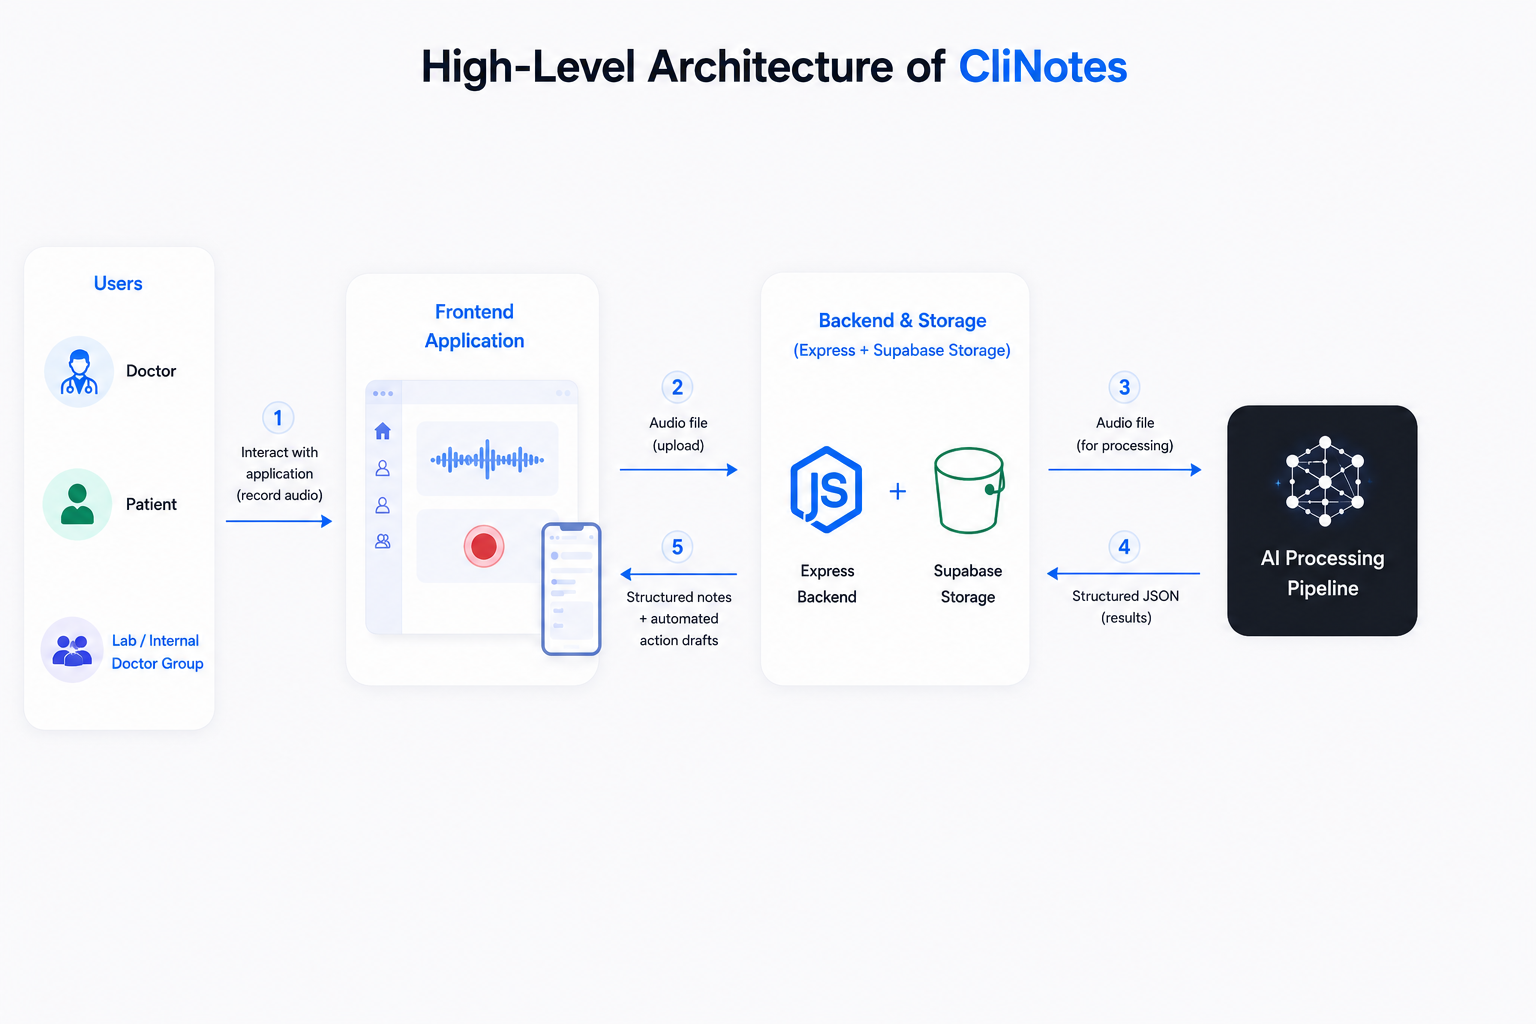
\includegraphics[width=0.98\textwidth]{highlvlarch.png}
  \caption{High-level CliNotes system architecture}
  \label{fig:high-level-architecture}
\end{figure}

As shown in Figure~\ref{fig:high-level-architecture}, the system is organized around three main workflow groups: doctors, patients, and internal doctor discussions. Doctors use the doctor dashboard to view schedules, access patient context, verify patients through the QR-based patient card, record consultations, review AI-generated drafts, and approve or discard recommended actions. Patients use the patient dashboard to book consultations, view reviewed consultation summaries, inspect transcripts, and display their patient card. The labs workflow allows multiple doctors to participate in a recorded internal discussion and later receive a generated discussion report.

The backend service is implemented in \texttt{server.js} using Node.js and Express. It exposes endpoints for raw audio upload, transcription triggering, transcript retrieval, test pipeline execution, patient-friendly summary generation, laboratory discussion processing, doctor discussion retrieval, patient Apple Wallet pass generation, and booked slot lookup. The Express layer acts as the trusted processing boundary of the system. It uses environment variables for private service credentials, including the Supabase service role key, Soniox API key, Gemini API key, and WalletWallet API key. This prevents the browser bundle from directly exposing secrets required for transcription, AI analysis, storage writes, or wallet pass generation.

The persistent data layer is Supabase. Supabase Auth manages user identity, while Supabase PostgreSQL stores profiles, doctors, patient profiles, consultations, audio metadata, transcripts, AI summaries, lab discussions, lab discussion participants, bookings, and related records. Supabase Storage stores consultation audio in the \texttt{consultation-audio} bucket and internal doctor discussion audio in the \texttt{lab-discussion-audio} bucket. The frontend uses the Supabase JavaScript client for authenticated reads and writes, while the Express backend uses the Supabase service role key for server-side workflows that must update storage objects, transcript rows, AI summary rows, and background processing status.

This high-level separation creates three important architectural boundaries. First, the browser remains responsible for interaction-heavy workflows such as recording, booking, dashboard rendering, and review. Second, Supabase provides identity, persistence, row-level access control, and file storage. Third, the Express backend centralizes privileged processing and all calls to Soniox, Gemini, and WalletWallet. As a result, audio and transcript processing are not performed directly by the client, and the user-facing pages receive only the processed states, drafts, summaries, and records required for the workflow.

\subsection{Stage 2: In-Depth AI Processing Layer}
\label{subsec:ai-processing-architecture}

The AI processing layer is the part of the architecture responsible for converting clinical audio into usable documentation. It is intentionally implemented on the backend because it requires access to private API keys, long-running orchestration, temporary external resources, JSON validation, and writes to protected database tables. This layer is used for both doctor-patient consultations and internal doctor discussions, with different transcription context and Gemini prompts for each mode.

\begin{figure}[H]
  \centering
  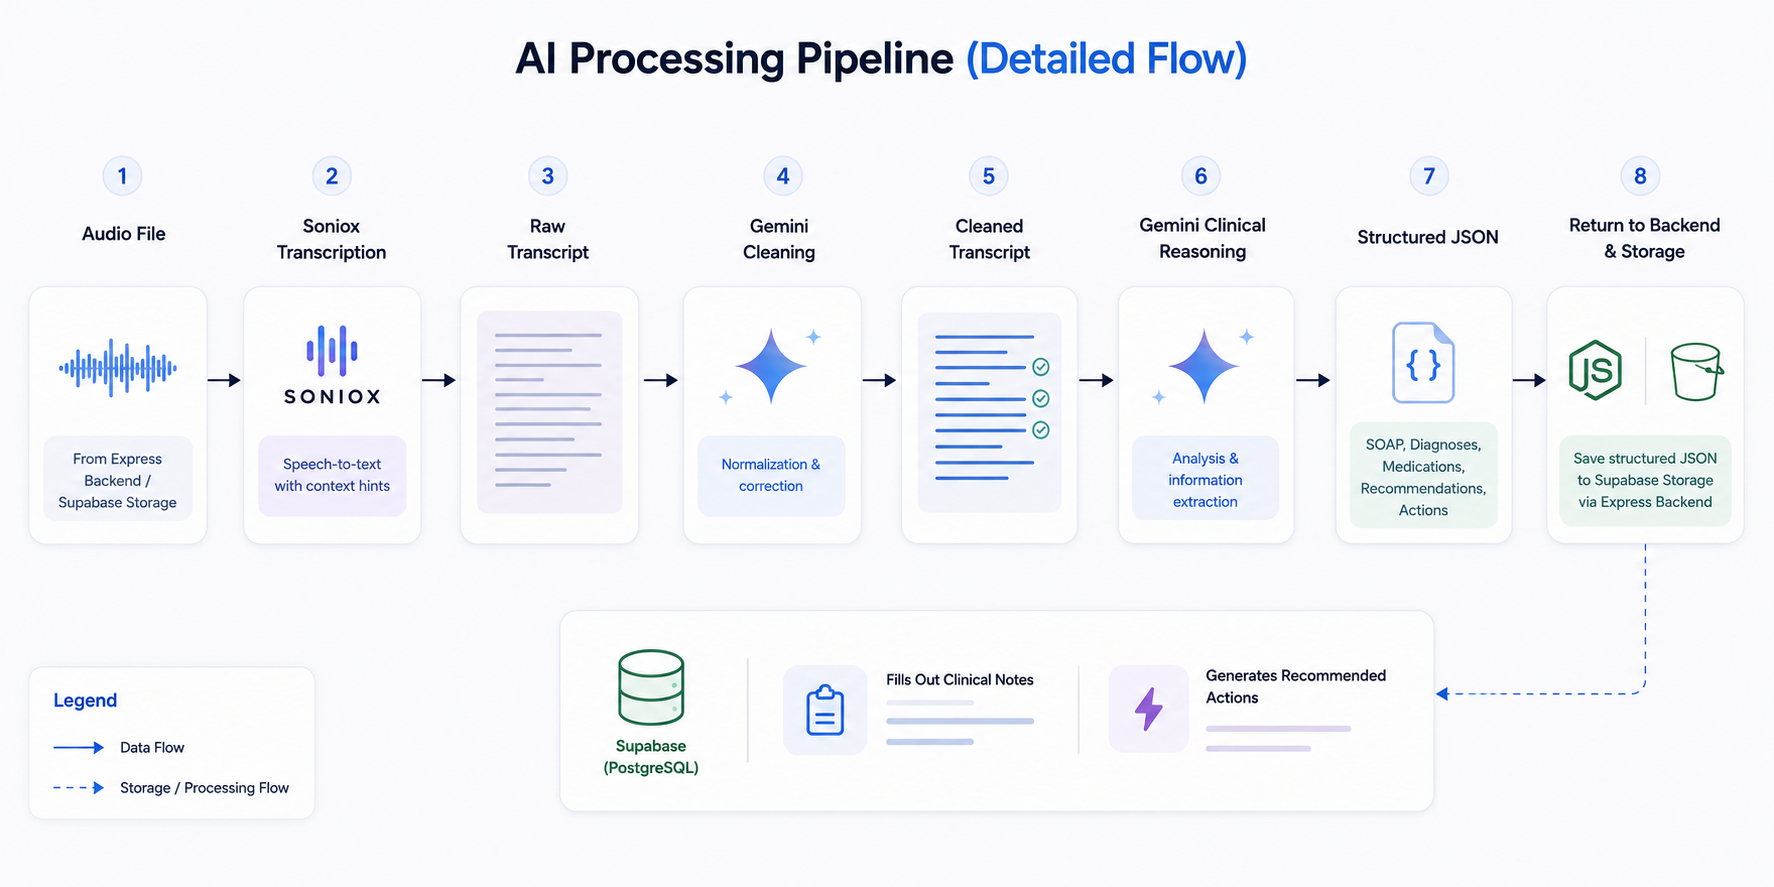
\includegraphics[width=0.98\textwidth]{indeptharch.png}
  \caption{In-depth architecture of the CliNotes AI processing layer}
  \label{fig:ai-processing-architecture}
\end{figure}

Figure~\ref{fig:ai-processing-architecture} shows the detailed flow through the AI pipeline. The process begins when audio is captured in the browser using the \texttt{MediaRecorder} API. For a patient consultation, the doctor dashboard creates a consultation record, records the encounter, and uploads the resulting WebM audio blob to the Express backend. For an internal discussion, the labs page records a doctor-to-doctor discussion and uploads it through the corresponding lab discussion endpoint. In both cases, the backend stores the audio in Supabase Storage and records metadata that links the stored file to the consultation or lab discussion.

After storage, the backend submits the audio to Soniox using the asynchronous \texttt{stt-async-v4} transcription model. The transcription configuration enables speaker diarization, language identification, and English-Arabic language hints. It also provides domain-specific context terms for medical conversations, including diagnoses, investigations, measurements, imaging names, and common medication terms. This configuration is important because the target use case includes Arabic sentences with English clinical terminology, and the transcription service must be guided to preserve those terms as accurately as possible.

When Soniox completes the transcription job, the backend retrieves both the plain transcript text and token-level information. Token data is rendered into a markdown transcript with speaker labels when speaker diarization is available. The plain transcript is then passed to Gemini for structured analysis. The active Gemini model is selected from the \texttt{GEMINI\_MODEL} environment variable and defaults to \texttt{gemini-3.5-flash}. The backend uses a structured prompt that asks Gemini to return strictly valid JSON rather than free-form text.

For doctor-patient consultations, Gemini is prompted to produce a clinical summary, SOAP-style structured data, four categories of recommended actions, patient-friendly explanation fields, and a lightly cleaned transcript. The recommended actions are limited to follow-up booking, prescription draft generation, lab or imaging order generation, and referral draft generation. The prompt explicitly instructs the model not to invent medications, tests, referrals, or follow-up timing that are not supported by the transcript. The cleaned transcript is expected to preserve the transcript order and meaning while correcting obvious transcription mistakes, especially English clinical terms that may have been transcribed phonetically in Arabic.

For internal doctor discussions, Gemini is prompted differently. Instead of SOAP notes, it generates a discussion headline, summary, prominent points, decisions, open questions, action plan, and cleaned transcript. The resulting report is routed back to the participating doctors for review before it is stored as an approved lab discussion. This keeps the lab workflow separate from patient consultation notes while reusing the same general audio-to-transcript-to-analysis pattern.

The backend validates the Gemini response before it is used. The helper \texttt{parseGeminiJsonResponse} extracts a JSON object from the model response and parses it. If the first parse fails, the backend calls \texttt{repairGeminiJson}, which asks Gemini to repair only the JSON syntax while preserving the clinical content. This repair step is included because long mixed-language transcript fields can occasionally produce malformed JSON when line breaks or quotation marks are not escaped correctly. After parsing, the backend derives the cleaned transcript, stores the AI summary in the \texttt{ai\_summary} table, updates the transcript row with the cleaned transcript, and marks the consultation or discussion as ready for review.

The final stage of the AI layer is human review. Generated consultation notes are not automatically published to the patient. They are shown to the doctor as draft notes for review. Only after approval does the system mark the consultation as reviewed and expose the final summary, patient-friendly explanation, transcript, and relevant actions to the patient-facing profile. This human-in-the-loop step is a deliberate architectural control that prevents unreviewed AI output from becoming part of the finalized patient record.

\section{Methodology and Processing Pipeline}
\label{sec:methodology-processing-pipeline}

The methodology implemented by CliNotes is a pipeline that transforms an audio consultation into a structured and reviewable medical record. The workflow is intentionally asynchronous after audio upload. This allows the doctor interface to return control to the user while transcription and analysis continue in the background. The doctor dashboard polls periodically when processing drafts are present, and processed consultations are later shown as drafts ready for clinical review. The implemented stages are described below.

\subsection{Stage 1: Patient Consultation Recording}
\label{subsec:stage-recording}

The objective of this stage is to create a consultation context and capture the audio evidence for the encounter. The stage starts when a doctor initiates a consultation from the dashboard. The patient may be selected by scanning a QR value that contains the patient identifier. When the consultation is started from a scheduled appointment, the scanned patient identifier is validated against the expected patient identifier for that booking. If the identifier does not match, the recording process is rejected and the doctor is asked to scan the correct patient card. The system also supports searching patient profiles by name and showing recent patient context before recording.

The inputs to this stage are the authenticated doctor session, the patient identifier, and the browser microphone stream. The implementation validates the doctor role when the doctor dashboard loads. It validates the patient identifier by attempting to create a consultation row through Supabase and by reading the patient profile after scanning. It validates microphone access by requesting audio permission through \texttt{navigator.mediaDevices.getUserMedia}. If the browser denies microphone access, the system stops the recording workflow and displays an error.

The processing steps are implemented in \texttt{src/doctor.js}. The doctor creates a new consultation row through \texttt{api.data.createConsultation}, which inserts the doctor identifier, patient identifier, and default consultation metadata into the \texttt{consultation} table. Once the consultation row exists, the browser starts \texttt{MediaRecorder} with one-second data intervals. Audio chunks are accumulated in memory while a timer is displayed in the recording overlay. When the doctor stops recording, the chunks are converted into an \texttt{audio/webm} blob. Before upload, the consultation status is set to \texttt{processing}. The audio blob is then sent to the Express endpoint \texttt{/api/upload-audio/:consultationId}.

The output of this stage is a consultation row in the \texttt{consultation} table, a WebM audio object uploaded through the backend, and a status transition from \texttt{pending} to \texttt{processing}. The Express backend stores the audio in the \texttt{consultation-audio} bucket under a path formed from the consultation identifier and a timestamp. It also inserts an \texttt{audio} metadata row that links the consultation to the storage file path.

\subsection{Stage 2: Speech Transcription}
\label{subsec:stage-transcription}

The objective of this stage is to convert the recorded consultation audio into machine-readable transcript text. After a successful upload, the frontend calls \texttt{api.data.triggerTranscription}, which sends the consultation identifier to the backend endpoint \texttt{/api/transcribe}. The endpoint validates that the Soniox API key and Supabase administrative client are configured, retrieves the latest audio file path for the consultation from the \texttt{audio} table, downloads the audio file from Supabase Storage, and inserts a \texttt{transcript} row with status \texttt{processing}.

The inputs to this stage are the consultation identifier, the stored audio file, the audio metadata row, and the Soniox configuration built by \texttt{buildTranscriptionConfig}. The transcription configuration uses the Soniox asynchronous model \texttt{stt-async-v4}. It enables speaker diarization, enables language identification, and supplies English and Arabic language hints. It also provides medical context terms such as common diagnoses, tests, scans, measurements, and medication names. The implementation therefore explicitly supports Arabic-English code switching at the transcription configuration level by informing Soniox that both languages may appear and by supplying a clinical context that includes English medical terminology in otherwise Arabic speech.

The processing steps are asynchronous. The backend returns a response to the frontend immediately after creating the processing transcript row. In the background, it uploads the audio buffer to Soniox, creates a transcription job, saves the returned Soniox transcription identifier into the \texttt{transcript} table, polls the Soniox job until completion or timeout, and retrieves the final transcript with token-level information. The token stream is rendered into markdown by grouping text by speaker identifier when speaker diarization is present. The plain transcript text is also retained for Gemini analysis.

The output of this stage is a raw transcript from Soniox, a markdown transcript with speaker labels when available, Soniox metadata such as audio duration, and a \texttt{transcript} table row that is later updated with either completed transcript data or an error message. The implementation deletes temporary Soniox transcription and file resources after processing succeeds or fails.

\subsection{Stage 3: Clinical Information Extraction}
\label{subsec:stage-clinical-extraction}

The objective of this stage is to transform the transcript into structured clinical documentation. Once the Soniox transcript is available, the backend calls \texttt{analyzeTranscriptWithGemini} if Gemini is configured and the transcript contains usable text. The Gemini prompt instructs the model to produce strictly valid JSON containing a short summary, a structured SOAP note, recommended actions, patient-facing summary fields, and a cleaned transcript.

The inputs to this stage are the raw transcript text, the Gemini system instruction, the configured Gemini model, and the expected JSON schema encoded in the prompt. The output format requested by the implementation contains \texttt{summary\_text} and a \texttt{structured\_data} object. The structured object includes title, subjective information, objective information, assessment, plan, recommended actions, patient summary fields, and cleaned transcript text. The recommended action object supports four action types: follow-up, prescription, lab or imaging order, and referral. The prompt explicitly instructs the model not to invent medications, tests, referrals, or follow-up timing when they are not supported by the transcript.

The processing steps include model invocation, JSON extraction, JSON parsing, and repair if the first model response is syntactically invalid. The function \texttt{parseGeminiJsonResponse} extracts a JSON object from the model response. If parsing fails, \texttt{repairGeminiJson} asks Gemini to repair only the JSON syntax while preserving the medical content. The cleaned transcript is obtained from the Gemini output when available and is normalized for mixed Arabic-English display by wrapping recognized medical terms in square brackets inside Arabic lines. A cleaned markdown transcript is then produced for display.

The output of this stage is an AI-generated draft consisting of a summary, SOAP-like structured data, recommended action candidates, patient-friendly explanation fields, and a cleaned transcript. The summary is stored in the \texttt{ai\_summary} table. The cleaned transcript is written back into the \texttt{transcript} table. The consultation status is later updated to \texttt{processed}, indicating that the draft is ready for doctor review.

\subsection{Stage 4: Data Persistence}
\label{subsec:stage-persistence}

The objective of this stage is to persist each artifact generated by the consultation pipeline in a retrievable and relationally consistent form. The database operations are split between browser-side Supabase calls and backend service-role calls. The browser creates consultations, updates statuses, creates bookings, retrieves records, and updates reviewed summaries according to RLS policies. The backend handles storage upload, audio metadata insertion, transcript creation, transcript updates, AI summary insertion, and background status changes.

The inputs to this stage are the consultation identifier, doctor identifier, patient identifier, audio file path, Soniox transcription identifier, transcript text, markdown transcript, AI summary, structured JSON, and status values. The main tables involved are \texttt{consultation}, \texttt{audio}, \texttt{transcript}, and \texttt{ai\_summary}. The \texttt{consultation} table acts as the parent record. The \texttt{audio}, \texttt{transcript}, \texttt{ai\_summary}, \texttt{doctor\_recommendation}, and \texttt{highlight} tables reference \texttt{consultation} through foreign keys. The \texttt{consultation} table itself references \texttt{doctor} and \texttt{patient\_profile}.

The processing steps begin with insertion of a consultation row. The audio upload endpoint writes the WebM file to the \texttt{consultation-audio} bucket and records the path in the \texttt{audio} table. The transcription endpoint creates a \texttt{transcript} row in the \texttt{processing} state, updates it with the Soniox transcription identifier, and then updates it with transcript text, markdown, and status \texttt{completed}. If an error occurs during background processing, the transcript status becomes \texttt{error} and the error message is stored. AI analysis results are inserted into \texttt{ai\_summary}. Finally, the consultation status is set to \texttt{processed}. During doctor review, the edited structured data is written back into \texttt{ai\_summary}, and the consultation status is changed to \texttt{reviewed}.

The output of this stage is a persisted clinical record that can be retrieved by the doctor dashboard, patient profile page, and patient dashboard. Security considerations at this stage include database-level RLS, user role checks in several backend routes, and the use of the service role key only on the server. A limitation of the current implementation is that some privileged endpoints do not verify a bearer token before accepting identifiers and processing data. This means that the deployment environment must protect the backend and that additional route-level authorization should be added before production use.

\subsection{Stage 5: Clinical Review Interface}
\label{subsec:stage-review-interface}

The objective of this stage is to keep the physician responsible for the final clinical record. The system does not automatically publish the AI-generated note to the patient as a final record. Instead, processed consultations appear in the doctor dashboard as drafts marked ready for review. The doctor opens a review modal, inspects the structured data, may edit the fields, and then approves the note.

The inputs to this stage are the processed consultation row, joined patient and doctor data, the \texttt{ai\_summary} row, and the structured JSON produced by Gemini. The doctor dashboard loads consultations using \texttt{api.data.getConsultations}, which selects consultations together with related doctor, patient, and AI summary data. It calculates dashboard metrics for scheduled visits, processing consultations, ready drafts, and reviewed consultations. It also displays processing rows and polls the backend state periodically when processing items exist.

The processing steps in the review interface are implemented mainly in \texttt{src/doctor.js}. The review modal maps structured JSON fields into editable form controls for title, chief complaint, history, allergies, vitals, physical examination, diagnoses, treatment, and follow-up. When the doctor approves the note, the frontend reconstructs the structured JSON from the edited fields. If no patient summary exists, the frontend requests generation of a patient-friendly summary through \texttt{/api/patient-summary}, which verifies the bearer token and doctor role before calling Gemini. The final structured data is then saved with \texttt{api.data.updateAISummary}, and the consultation is marked \texttt{reviewed}.

The output of this stage is a reviewed consultation record. Reviewed consultations appear in the doctor's history and in the patient's dashboard. The patient dashboard deliberately filters consultations to reviewed records, preventing unreviewed AI drafts from appearing in the patient-facing interface. Patients can view summary tiles and, when available, the completed transcript for reviewed consultations.

\subsection{Stage 6: Recommended Actions Engine}
\label{subsec:stage-recommended-actions}

The objective of this stage is to convert supported clinical plan items into actionable drafts that remain under physician control. The engine is implemented partly in the Gemini prompt and partly in frontend logic. Gemini is instructed to return a \texttt{recommended\_actions} object containing follow-up, prescription, lab order, and referral candidates, but only when they are clearly supported by the consultation transcript. The frontend then interprets pending recommended actions and renders them in the doctor dashboard.

The inputs to this stage are the \texttt{structured\_data.recommended\_actions} object, consultation metadata, patient name, doctor name, and consultation date. Each action contains a \texttt{needed} flag and a \texttt{status}, initially expected to be \texttt{pending}. Follow-up actions may include timing and reason. Prescription actions may include medication name, dose, frequency, duration, and instructions. Lab order actions may include order type, name, reason, and priority. Referral actions may include specialty, reason, and debrief information.

The processing steps are implemented in \texttt{getGeneratedRecommendedActions}, \texttt{renderRecommendedActionForm}, and related helper functions in \texttt{src/doctor.js}. Pending actions are shown as dashboard rows. When opened, a modal renders an editable form corresponding to the action type. Follow-up approval creates a new booking row for the patient using \texttt{api.data.createDoctorBooking}; the system infers a default date from the timing text when possible and otherwise defaults to a later appointment. Prescription, lab order, and referral actions are not persisted as separate normalized database rows in the current implementation. Instead, they are edited, printed through a browser print window, and their approved or discarded status is written back into the nested \texttt{structured\_data.recommended\_actions} object in \texttt{ai\_summary}.

The output of this stage is either a follow-up booking record or a printable reviewed action document. In all cases, the action status is updated inside the AI summary JSON. This design provides a practical lightweight action workflow, but it also means that prescriptions, lab orders, and referrals are not represented as independent database entities in the current schema.

\section{Database Design}
\label{sec:database-design}

The database design is centered on Supabase PostgreSQL and Supabase Auth. Application user records are normalized into a base profile table and role-specific tables. Clinical records are centered on the \texttt{consultation} table, which connects a doctor and a patient. Generated artifacts such as audio metadata, transcripts, summaries, recommendations, and highlights are associated with consultations. Separate tables support internal doctor discussions and appointment booking.

The \texttt{profiles} table contains one row per authenticated application user. Its primary key is \texttt{id}, which references \texttt{auth.users(id)} with cascading deletion. It stores \texttt{role}, constrained to \texttt{doctor} or \texttt{patient}, and \texttt{created\_at}. The inspected schema does not include a \texttt{labs} role in this table, even though the login UI contains a labs entry path. Therefore, the labs workflow should be understood as a doctor-oriented subsystem rather than a separate persisted user role.

The \texttt{doctor} table stores doctor-specific user data. Its primary key \texttt{id} references \texttt{profiles(id)}. It contains a unique \texttt{doctor\_id}, a required \texttt{name}, an optional \texttt{specialty}, and \texttt{created\_at}. The table is used by consultation joins, available doctor listing, booking workflows, and lab discussion participant verification.

The \texttt{patient\_profile} table stores patient-specific profile data. Its primary key \texttt{id} references \texttt{profiles(id)}. It contains \texttt{name}, \texttt{age}, \texttt{gender}, and \texttt{created\_at}. It is used for patient dashboards, doctor search, patient history display, bookings, and QR-card identification.

The \texttt{consultation} table is the main clinical encounter table. Its primary key is \texttt{id}, generated by \texttt{uuid\_generate\_v4()}. It references \texttt{doctor(id)} through \texttt{doctor\_id} and \texttt{patient\_profile(id)} through \texttt{patient\_id}. It also contains \texttt{date\_time}, \texttt{duration}, \texttt{status}, and \texttt{created\_at}. The \texttt{status} field is constrained to \texttt{pending}, \texttt{processing}, \texttt{processed}, or \texttt{reviewed}. This status field is used by the frontend to separate active drafts, processed drafts, and finalized consultations.

The \texttt{audio} table stores metadata for consultation audio files. Its primary key is \texttt{id}. It references \texttt{consultation(id)} through \texttt{consultation\_id}. It contains \texttt{file\_path}, \texttt{duration}, and \texttt{created\_at}. The actual audio bytes are stored in Supabase Storage, not in the relational table.

The \texttt{ai\_summary} table stores AI-generated and doctor-edited summary data. Its primary key is \texttt{id}. It references \texttt{consultation(id)} through \texttt{consultation\_id}. It contains \texttt{summary\_text}, \texttt{structured\_data} as JSONB, and \texttt{created\_at}. The JSONB field stores SOAP fields, patient summary fields, recommended actions, and cleaned transcript data as returned or later edited by the application.

The \texttt{doctor\_recommendation} table stores free-text doctor recommendation data. Its primary key is \texttt{id}, and it references \texttt{consultation(id)}. It contains \texttt{recommendations\_text} and \texttt{created\_at}. The inspected frontend reads this table in patient profile history, but the main recommended action engine currently stores statuses inside \texttt{ai\_summary.structured\_data} rather than inserting separate rows here.

The \texttt{highlight} table stores smart moment capture metadata. Its primary key is \texttt{id}, and it references \texttt{consultation(id)}. It contains \texttt{start\_time}, \texttt{end\_time}, \texttt{label}, and \texttt{created\_at}. The schema and dashboard contain traces of a capture feature, but the inspected implementation does not show complete persistence logic for creating highlight rows during a recording. This chapter therefore treats it as a defined but only partially implemented feature.

The \texttt{transcript} table stores transcription artifacts for consultations. Its primary key is \texttt{id}, and it references \texttt{consultation(id)}. It contains \texttt{transcript\_text}, \texttt{transcript\_markdown}, \texttt{soniox\_transcription\_id}, \texttt{status}, \texttt{error\_message}, and \texttt{created\_at}. The \texttt{status} field is constrained to \texttt{pending}, \texttt{processing}, \texttt{completed}, or \texttt{error}. This table allows the frontend to display transcript status and retrieve completed transcripts.

The \texttt{lab\_discussion} table stores internal doctor discussion records. Its primary key is \texttt{id}. It contains \texttt{title}, \texttt{audio\_path}, \texttt{transcript\_text}, \texttt{transcript\_markdown}, \texttt{soniox\_transcription\_id}, \texttt{summary\_text}, \texttt{structured\_data} as JSONB, \texttt{status}, \texttt{error\_message}, and \texttt{created\_at}. The status values are \texttt{pending}, \texttt{processing}, \texttt{processed}, \texttt{reviewed}, and \texttt{error}. This table parallels the consultation pipeline but is designed for internal doctor-to-doctor discussions rather than doctor-patient encounters.

The \texttt{lab\_discussion\_participant} table implements the many-to-many relationship between lab discussions and doctors. Its primary key is \texttt{id}. It references \texttt{lab\_discussion(id)} through \texttt{discussion\_id} and \texttt{doctor(id)} through \texttt{doctor\_id}. It includes \texttt{approved\_at} and \texttt{created\_at}, and it enforces uniqueness over \texttt{discussion\_id} and \texttt{doctor\_id}. A doctor approves their participation or review by updating the \texttt{approved\_at} field.

The \texttt{booking} table stores appointment bookings. Its primary key is \texttt{id}. It references \texttt{doctor(id)} and \texttt{patient\_profile(id)}. It contains \texttt{appointment\_time}, \texttt{reason\_text}, \texttt{reason\_audio\_path}, \texttt{status}, and \texttt{created\_at}. Booking status is constrained to \texttt{scheduled}, \texttt{completed}, \texttt{cancelled}, or \texttt{no\_show}. Patients create bookings through the patient dashboard, and doctors can update scheduled bookings when a patient is completed, cancelled, or marked as no-show.

\noindent\textbf{[FIGURE PLACEHOLDER: Entity Relationship Diagram]}

The ERD should contain \texttt{auth.users} at the top, connected one-to-one to \texttt{profiles}. From \texttt{profiles}, draw one-to-one subtype relationships to \texttt{doctor} and \texttt{patient\_profile}. Draw \texttt{doctor} and \texttt{patient\_profile} as parents of \texttt{consultation}, where each consultation belongs to one doctor and one patient. Draw one-to-many relationships from \texttt{consultation} to \texttt{audio}, \texttt{transcript}, \texttt{ai\_summary}, \texttt{doctor\_recommendation}, and \texttt{highlight}. Draw \texttt{booking} as a junction-like appointment table connected to one doctor and one patient. Draw \texttt{lab\_discussion} connected many-to-many with \texttt{doctor} through \texttt{lab\_discussion\_participant}. Mark all primary keys as UUIDs and show the foreign keys exactly as described: \texttt{doctor.id -> profiles.id}, \texttt{patient\_profile.id -> profiles.id}, \texttt{consultation.doctor\_id -> doctor.id}, \texttt{consultation.patient\_id -> patient\_profile.id}, and all consultation artifact foreign keys pointing to \texttt{consultation.id}.

\section{Security and Privacy Considerations}
\label{sec:security-privacy}

The system uses Supabase Auth as its authentication mechanism. Login is performed through email and password using \texttt{signInWithPassword}. Signup is performed through \texttt{signUp}, with metadata identifying the user's role and role-specific attributes. A PostgreSQL trigger named \texttt{on\_auth\_user\_created} executes \texttt{handle\_new\_user} after a new Supabase Auth user is inserted. This trigger creates a row in \texttt{profiles} and then inserts into either \texttt{doctor} or \texttt{patient\_profile} depending on the supplied role metadata. This design avoids client-side insertion into protected role tables during registration.

Authorization is implemented through a combination of frontend role guards, Supabase Row Level Security, and selected backend bearer-token checks. Frontend role guards redirect users away from dashboards that do not match their stored role. These guards improve usability but are not sufficient as a security mechanism by themselves. The primary database protection is RLS. The schema enables RLS on all application tables and defines policies for profile access, doctor records, patient profiles, consultations, audio metadata, AI summaries, doctor recommendations, highlights, transcripts, lab discussions, lab discussion participants, and bookings.

The RLS model permits patients to view their own records, including their profile, consultations, summaries, recommendations, highlights, transcripts, and bookings. Doctors can manage their own consultations and related artifacts. Additional policies allow authenticated doctors to search patient profiles and view patient consultations, summaries, recommendations, and transcripts. This broader doctor access supports the patient search and patient profile features, but it is less restrictive than a policy that limits doctors only to patients with existing appointments or consultations. The current authorization model therefore favors clinical usability and dashboard access over a strict minimum-access model.

The backend stores sensitive service credentials only on the server. The Supabase service role key, Soniox API key, Gemini API key, and WalletWallet API key are read from environment variables. This prevents the browser bundle from directly exposing these secrets. The backend uses the Supabase service role key to bypass RLS for storage uploads and background processing. This is necessary for the current architecture because the server must update database rows after asynchronous transcription and AI analysis. It also means the backend must be treated as a trusted component and must carefully validate requests.

Several medical data protection measures are present in the implementation. Audio files are stored in Supabase Storage rather than embedded in database rows. Consultation status gates patient visibility: the patient dashboard displays only consultations marked as \texttt{reviewed}. AI-generated summaries are placed in a doctor review workflow before being shown as finalized records. The Gemini prompt instructs the model not to invent facts and to include only actions supported by the transcript. Completed transcripts and summaries are retrieved through authenticated Supabase queries subject to RLS policies.

There are also implementation limitations that should be explicitly acknowledged. The upload and transcription endpoints for consultations do not currently verify an authenticated bearer token or confirm that the requester is the doctor associated with the consultation. The lab discussion creation and audio upload endpoints similarly rely on supplied identifiers and server-side service-role access. Some lab routes and patient-summary routes do validate the bearer token and role. For production deployment, the same validation pattern should be applied consistently to all privileged endpoints. Furthermore, storage policy definitions in the SQL files are explicit for \texttt{consultation-audio}, while the \texttt{lab-discussion-audio} bucket is created dynamically by server logic without a corresponding policy definition in the inspected schema. These issues do not prevent describing the implemented prototype, but they are relevant privacy and security considerations for a system handling clinical data.

\section{Design Rationale}
\label{sec:design-rationale}

The chosen architecture reflects a pragmatic separation between interactive clinical workflows, persistent medical data, and external AI processing. A Vite-based frontend with plain JavaScript modules is sufficient for the current application because each page is relatively self-contained and maps clearly to one user workflow. The doctor dashboard, patient dashboard, patient profile page, labs page, and test page are independent surfaces. This reduces framework complexity and allows the implementation to load only the JavaScript needed for each page. The tradeoff is that state management and UI composition are handled manually, which can become harder to maintain as the number of workflows grows.

The Express backend was adopted as a lightweight orchestration layer. It provides a place to keep API keys secret, receive raw audio uploads, communicate with Soniox and Gemini, use the Supabase service role safely on the server side, and run asynchronous background work after returning a response to the frontend. This design is particularly appropriate for audio transcription because the browser should not directly hold transcription API credentials and should not be responsible for long-running polling against a speech-to-text service. The current background processing is implemented inside the Node.js process itself rather than through a queue. This is simple and suitable for a prototype or low-volume deployment, but a production system would benefit from a durable job queue so that long-running transcription jobs survive server restarts.

Supabase was selected as the main backend infrastructure because it combines authentication, PostgreSQL, Row Level Security, storage, and a JavaScript client in one platform. This reduces the amount of custom backend code needed for ordinary authenticated CRUD operations. PostgreSQL is well suited to the relational parts of the system, such as doctors, patients, consultations, bookings, and participant relationships. JSONB is used in \texttt{ai\_summary.structured\_data} and \texttt{lab\_discussion.structured\_data} because AI outputs are semi-structured and may evolve more quickly than fixed relational columns. This choice improves flexibility during prototype development, although heavily used clinical action types may later require normalized tables for stronger validation, querying, auditing, and reporting.

Soniox was selected in the implemented pipeline for speech transcription because the application requires asynchronous audio transcription, speaker diarization, language identification, and Arabic-English code-switching support. The configuration explicitly supplies English and Arabic language hints and medical vocabulary context. These design choices are consistent with the target consultation environment, where Arabic conversation may contain English clinical terminology. Gemini was selected for the information extraction stage because the application requires structured JSON generation, transcript cleaning, SOAP summarization, patient-friendly explanation, and recommended action extraction from unstructured transcript text. The prompt constrains the model to output valid JSON and to avoid unsupported clinical inventions. The implementation also includes a repair step for invalid JSON, which improves robustness against occasional malformed model output.

Scalability is addressed partially through asynchronous processing and managed services. Supabase handles authentication, storage, database persistence, and RLS. Soniox and Gemini handle computationally expensive transcription and language analysis externally. The frontend is static and can be served efficiently. However, the current Express background processing model has scalability limits because transcription work runs inside the same server process that handles HTTP requests. Under higher load, this should be replaced or supplemented by a job queue, worker process, retry policy, and persistent job state beyond the existing transcript status fields.

Maintainability is supported by centralizing browser data access in \texttt{src/api.js}, separating page-specific behavior into page-specific modules, and keeping the AI orchestration in \texttt{server.js}. The schema is explicit and migration files document the incremental addition of transcription, patient booking, patient search, lab discussions, and booking no-show support. The main maintainability risk is that \texttt{server.js} contains many responsibilities in a single file, including transcription helpers, Gemini prompts, storage upload logic, lab routes, booking routes, and wallet pass generation. As the system grows, this file should be separated into route modules and service modules. Similarly, the recommended actions engine currently stores workflow state inside nested JSON rather than normalized action tables, which is practical for early development but less ideal for auditability and long-term clinical workflow management.

Overall, the implemented design is a prototype-oriented but coherent architecture for transforming consultation audio into reviewed clinical documentation. It uses managed infrastructure for identity, persistence, and storage, external AI services for transcription and information extraction, and a human review interface to prevent direct publication of unverified AI output. The most important future architectural improvements are stronger route-level authorization, durable background jobs, normalized clinical action records, and stricter storage policy definitions for all audio buckets.
